% Ötödik előadás

\chapter{Az AMD Zen processzorai}

\section{Bevezetés}
Az AMD a korábbi lemaradás után az utóbbi években újra felzárkózott az Intelhez és több kategóriában megverte őket teljesítményben.
A Zen elnevezés vonatkozhat általánosan a Zen mikroarchitektúrára épülő processzorokra és az első generációs Zen CPU-kra is.
A fejezetben ezért az első generációs Zeneknél explicit jelöljük a generációt.
A gyártó a mobil elnevezést a laptop processzorokra használja.

\section{Áttekintés}
Az 1960-as években a Fairchild Semiconductor vállalatból több cég kivált, de ezek közül csak az Intel és az AMD nem olvadt be más cégekbe.
Napjainkban ez a kettő határozza meg az x86 alapú processzorgyártást.

Az AMD először az Inteltől licenszelt processzorokat gyártott, 1996-ban a K5 processzorokkal jelentek meg a saját fejlesztésű termékeik.
A K8 a világ első 64 bites processzora volt (2003).
Ezután több, nem túl sikeres processzort gyártottak (Bulldozer, Cat), az újabb siker 2017-ben jött a Zen családdal.

Az AMD jelentőségteljes fejlesztései közé tartozik az x86-os utasításkészlet 64 bites kiterjesztése.
Ekkor az Intel és a HP 64 bites VLIW architektúrával próbálkozott (Itanium), az AMD viszont a meglévő x86-os architektúra kiterjesztésében látta a jövőt.
Ebből az AMD került ki győztesen.
A 64 bit megvalósításához ki kellett terjeszteni a regisztereket és az utasításokat is ki kellett bővíteni.

Az AMD másik fontos fejlesztése a DCA (Direct Connect Architecture) multiprocesszoros megoldás.
Ezzel a korábban az északi hídon lévő memóriavezérlőt integrálták a processzorlapkára, kiküszöbölve a memória szűk keresztmetszetét (főleg szervereknél volt probléma).
A DCA része még a HyperTransport link, amiből minden processzorra kerül három és a processzorok összekötését szolgálják.

A fejlesztéseknek köszönhetően az AMD 2003-ban megjelent processzorai teljesítményben jobbak voltak az Inteleknél.
Így egyre nagyobb piacot tudott magának szerezni.
Az Intel csak később vette át ezeket az újításokat, de végül ők is rákényszerültek az x86 64 bites kiterjesztésére (2004).
A lapkára integrált memóriavezérlőt viszont csak 2008-ban hozta be az Intel a Nehalem processzorokkal.

Az AMD piaci részesedése viszont 2006-tól csökkenni kezdett, mikor az Intel kihozta a Core 2 processzorait és az AMD elé került teljesítményben.
Ez a tendencia 2017-ben fordult meg, az AMD Zen processzorok megjelenésével.
A Zennel nagy mértékű teljesítmény és hatékonyság növekedést értek el, 2021 elején egymagos teljesítményt nézve az AMD Ryzen 9 5900X volt a leggyorsabb asztali processzor.

A szervereknél szintén az AMD EPYC processzorok vezetik a benchmarkokat.
Az Intel eléggé elmarad, viszont közben megjelentek az ARM alapú szerverek, amik teljesítményben majdnem elérik az AMD-t.
Az ARM architektúrák teljesítmény felvételben kedvezőbbnek tűnnek, tehát valós konkurencia az x86-nak.

\section{A Zen család tervezési elvei}
Az AMD 300 mérnöke dolgozott a Zen mikroarchitektúrán, hogy teljesítményben legyőzzék az Intelt.
A megvalósítási alapelvek:
\begin{itemize}
    \item többlapkás megközelítés
    \item lego-jellegű rendszer, három különböző lapkatípusból lehet összerakni a processzorokat:
    \begin{itemize}
        \item CPU lapkák
        \item APU lapkák - számítási és grafikai feldolgozást is megvalósít
        \item IO lapkák
    \end{itemize}
    \item három szintű hierarchikus tervezés
    \item a lapkák összekötéséhez szükséges egy új kapcsolóhálózat kifejlesztése, ez lett az Infinity Fabric (IF)
    \item a lapkákat egybe kell tokozni, ehhez egy két dimenziós tokozást alkalmaztak (MCM - Multi Chip Module)
\end{itemize}

\subsection{Többlapkás felépítés}
Korábban a processzorokat monolitikusan tervezték, azaz minden mag egy lapkára került.
Ilyen az Intel Skylake-SP (2017) is, ami 28 magot tartalmaz egy lapkán.
Az AMD EPYC (2017) viszont többlapkás megvalósítást használ, négy, egyenként nyolc magos lapkát tartalmaz egy tokozásban (\ref{fig:multidie}).
\begin{figure}[H]
    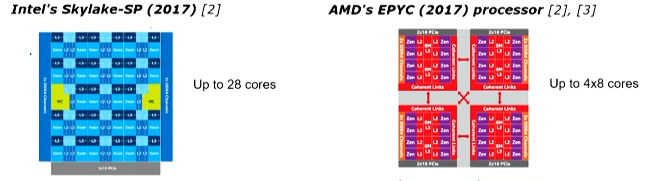
\includegraphics[width=0.8\textwidth]{multidie}
    \centering
    \caption{Monolitikus és többlapkás felépítés}
    \label{fig:multidie}
\end{figure}
A többlapkás felépítés fő előnye, hogy kisebb lapkák gyártásával kisebb a hibaarány, így nagyobb lesz a kihozatal, tehát a gyártás költséghatékonyabb.
Az AMD becslése szerint egy 32 magos processzornál a többlapkás felépítés gyártási költsége mindössze 60\%-a az egylapkás felépítésűnek.
További előny, hogy ugyanazokból az alapelemekből több processzort is ki lehet alakítani, valamint a memória csatornák és az IO skálázható a magok számával.

Hátrány viszont, hogy egy cache koherens összekapcsoló hálózat kell, ami csökkenti a teljesítményt és növeli a fogyasztást.
Ezen kívül a tokozás növeli a gyártási költségeket.

A többlapkás felépítést az Intel is tervezi átvenni, valamint az Nvidia is végez kutatásokat a GPU-k többlapkás felépítésével kapcsolatban.

\subsection{Moduláris kialakítás}
A teljes Zen család három fajta lapkából épül fel (CPU, APU és IO).

A CPU lapkák nem tartalmaznak GPU-t.
Az első generációban Zeppelinnek, később CCD-nek (CPU Compute Dies) hívták.
Az APU lapkák CPU-t és integrált GPU-t is tartalmaznak, az IO lapkák pedig az IO-ért felelnek.
IO lapkáknál megkülönböztetünk szerverekben és HEDT gépekben használt IOD-okat (IO Dies) és kliensekben használt cIOD-okat (Client IO Dies).

Az asztali processzorok, a HEDT-ek és a szerverek nem tartalmaznak grafikát, több lapkából állnak és tartalmaznak IO lapkát is.
Ezzel szemben a laptopokba és asztali gépekbe szánt APU-k egy lapkás SoC-ok, GPU-t is tartalmaznak.
A különböző lapkatípusokat mutatja be a \ref{fig:die}. ábra.

\begin{figure}[H]
    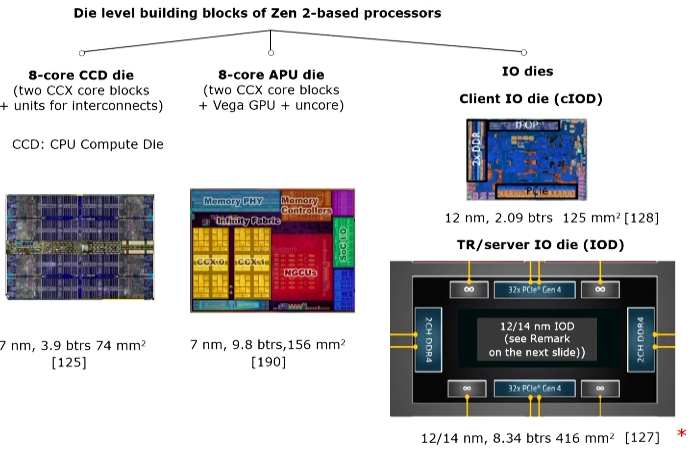
\includegraphics[width=0.8\textwidth]{die}
    \centering
    \caption{A Zen 2 processzorokat alkotó lapkák}
    \label{fig:die}
\end{figure}

A mobil és desktop APU-k egy APU lapkából állnak, legfeljebb 8 maggal (Ryzen 4xxU/H/HS és Ryzen 4xxG/GE).
A GPU nélküli desktopok (Ryzen 3xxx/X) 1 vagy 2 CCD lapkát és 1 cIOD lapkát tartalmaznak (max 16 mag).
24 és 32 magos HEDT processzoroknál 4 darab 6 vagy 8 aktivált magos CCD és 1 IOD lapka van a foglalatban, 64 magnál pedig 8 darab 8 magos CCD és 1 IOD (Threadripper 39xxX).
Szervereknél 24 és 32 mag esetében 4 darab 4 vagy 6 magos CCD és 1 IOD, 48 és 64 magnál pedig 8 darab 4 vagy 6 magos CCD és 1 IOD dolgozik.

\subsection{A CPU-k és GPU-k három szintű hierarchikus tervezése}
Az AMD a CPU és GPU lapkákat hierarchikus módon tervezte.
Jelentése, hogy az alap építőkocka a mag, a magok összerakásából funkcionális egységek építhetők, a funkcionális egységekből pedig lapkák.

Ezek az építőkockák:
\begin{itemize}
    \item CPU: CPU magok, CPU mag blokkok, CPU lapkák
    \item Grafika: GPU magok, GPU, APU lapka (egy GPU és egy vagy két CPU mag blokk)
    \item IO: csak kétféle lapka (HEDT/szerver és kliens)
\end{itemize}

\subsubsection{A CPU építőelemei}
A CPU magok a Zen processzorok alap építőelemei.
Ezekből alakulnak ki a CPU blokkok, amik 4 vagy 8 magot tartalmaz.
A magoknak saját L1 és L2 gyorsítótárai vannak, az L3 cache viszont osztott és szeletelt.
A szeletek egymás mellett párhuzamosan képesek dolgozni.
A magcsoportok neve CCV (Core CompleX).
A harmadik szint a lapka szint, a lapka egy vagy két CCX-et tartalmaz.
Az első generációs CPU-kat Zeppelin lapkáknak hívták, később CCD-re (Core Complex Dies) nevezték át.

Az Intel ezzel szemben nem magcsoportokat használt, hanem szimmetrikus többmagos rendszereket épített.
2020-ban az Intel viszont a Lakefield családdal áttért a magblokkok használatára és a big.little felépítésre, többlapkás felépítést használva.

A \ref{fig:zen1}. ábrán látható egy példa a CPU hierarchikus felépítésére.
\begin{figure}[H]
    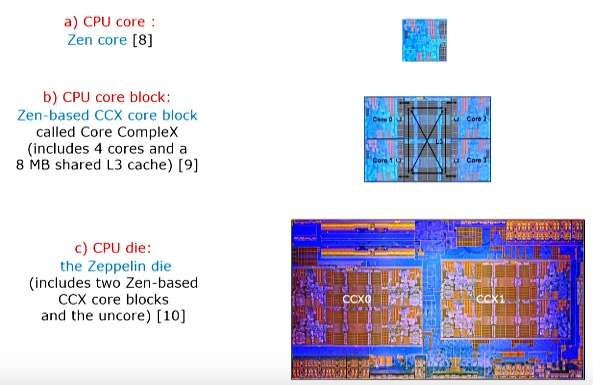
\includegraphics[width=0.8\textwidth]{zen1}
    \centering
    \caption{A Zen 1 processzorok felépítése}
    \label{fig:zen1}
\end{figure}

\subsubsection{A GPU építőelemei}
Itt az alap építőelem a GPU mag, ami megegyezik az AMD diszkrét videokártyáiban használt Vega CU-kkal (Compute Unit).
A második szint a Vega GPU-k amik 3-11 Vega CU-t tartalmaznak és egyéb szükséges egységeket.
Harmadik szinten az APU lapka van, ami egy Vega GPU-t és egy vagy két CCX-et tartalmaz.

Az APU-nak a GPU-n és CCX-en kívül szüksége van egyéb blokkokra a működéshez, ezeket összefoglalva uncore-nak nevezzük.

Egy APU felépítése látható a \ref{fig:vega}. ábrán.
A \ref{fig:vega}. ábrán látható egy példa a CPU hierarchikus felépítésére.
\begin{figure}[H]
    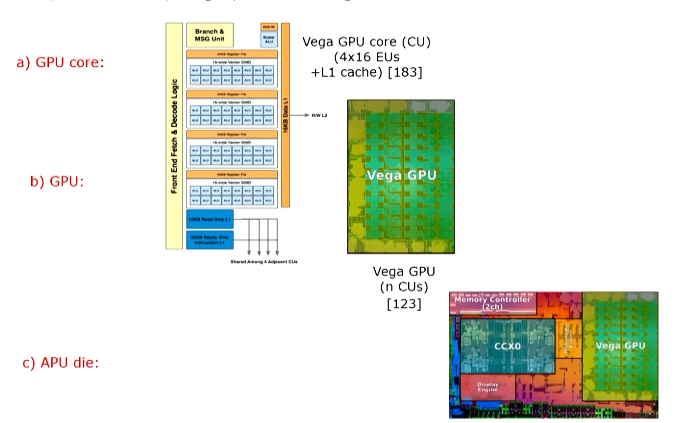
\includegraphics[width=0.8\textwidth]{vega}
    \centering
    \caption{Az APU SoC felépítése}
    \label{fig:vega}
\end{figure}

\subsection{A Zen magok fejlődése}
A Bulldozer processzorokhoz képest több téren előrelépést jelentett.
A Bulldozer magban két egész feldolgozó egységet integráltak egy lebegőpontos feldolgozóval és ezt a modult tekintették két magosnak.
Ez nem vált be, ezért a Zen visszatért a hagyományos mag felépítéshez (\ref{fig:bulldozervszen}).
\begin{figure}[H]
    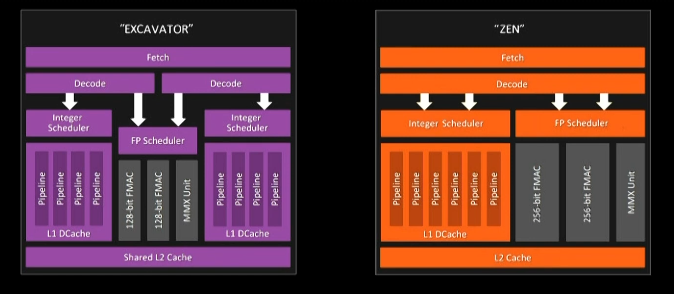
\includegraphics[width=0.8\textwidth]{bulldozervszen}
    \centering
    \caption{Különbség a Bulldozer alapú és a Zen architektúrák között}
    \label{fig:bulldozervszen}
\end{figure}
A Bulldozernek gyengéje volt még, hogy nem alkalmazott többszálúságot, a Zen viszont már megvalósította (\ref{fig:mt}).
\begin{figure}[H]
    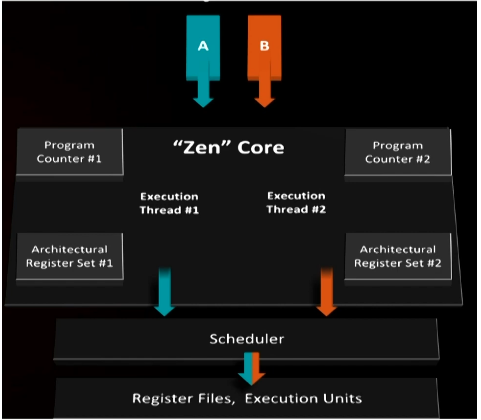
\includegraphics[width=0.6\textwidth]{mt}
    \centering
    \caption{Többszálúság a Zen magokban}
    \label{fig:mt}
\end{figure}
A harmadik nagy újítás egy olyan műszaki csomag volt, ami segített a disszipáció csökkentésében és a teljesítmény növelésében.
Az AMD ezt SenseMI-nak nevezte el és többek között adaptív feszültségszabályzást, Turbo Boostot, frekvencia növelést, neurális hálós elágazásbecslést és intelligens utasítás lehívást valósított meg.

Eredmények:
\begin{itemize}
    \item 14nm technológia a korábbi 28 helyett
    \item 52\%-os egyszálas teljesítmény javulás
    \item 3.7x-es javulás teljesítmény/wattban
    \item többszálúság
\end{itemize}

A Zen 1 után megjelent a Zen 2 és a Zen 3, 2022-re ígérik a Zen 4-et.
A Zen 2-nél 8-ról 16 MB-ra emelték az L3 cache-t és több, kisebb lapkát használtak fel.
A Zen 3 még tovább növelte az L3 méretét 32 MB-ra és itt már 4 helyett 8 magos komplexeket használtak.

\subsection{A CCX-ek fejlődése}
A Zen 1-nél 4 magos CCX-eket alkalmaztak (\ref{fig:zen1ccx}. ábra)
\begin{figure}[H]
    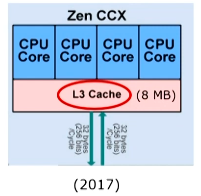
\includegraphics[width=0.4\textwidth]{zen1ccx}
    \centering
    \caption{Zen 1 CCX felépítése}
    \label{fig:zen1ccx}
\end{figure}
A magok saját L1 és L2 cache-el rendelkeztek.
A CCX 8 MB méretű közös L3 cache-t biztosít a magoknak, a külső komponensekkel pedig egy 32 byte széles, kétirányú linkkel kapcsolódik.
Az L3 cache négy darab 2 MB-os szeletre van osztva, amik cím átlapolással címezhetők.
A szeletek crossbar kapcsolattal kapcsolódnak, azaz bármelyik mag képes elérni bármelyik szeletet azonos időben (\ref{fig:crossbar}. ábra).
Ez többnyire exkluzív cache, tehát az L2-ből kimaradó adatokat tárolja (áldozat cache).
\begin{figure}[H]
    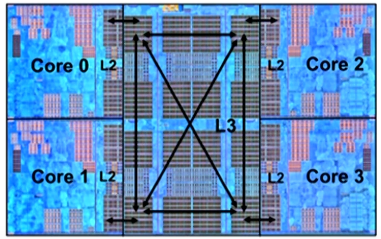
\includegraphics[width=0.5\textwidth]{crossbar}
    \centering
    \caption{Zen L3 cache felépítése}
    \label{fig:crossbar}
\end{figure}

Az ARMv8 ISA szintén magkomplexumokra épül, de megosztott L2 cache-t használ a Zennel ellentétben.
Később az ARM (8.2) már szintén privát L2 cache-t használt a magkomplexumoknál.
Ezeknél már megjelent a big.little architektúra is, azaz kis és nagy magokat kombinálhatnak a magkomplexumok.
Az AMD megvalósítása jobb volt mint az ARM 8.0, de elmarad a 8.2-től.

A Zen 2 architektúra megnövelte az L3 cache méretét, két CCX magblokkot tartalmaz és minden magblokknak 4 magja és 16MB L3 cache-e.
Itt a két cache összekötését meg kellett oldani, a Zen 3 viszont már közös 32 MB L3 cache-t biztosít a 8 magnak.
Ez csökkenti az elérési időket és a mag-mag futási időket.

\subsection{A grafikai magok fejlődése}
Az AMD a Vega számítási egységeit használta fel a Zen processzorokban.
